\chapter{Full EAToF data sets\label{ch:fulldata}}

\section{LCO pouch cell}

\begin{figure}[htb]
  \centering
    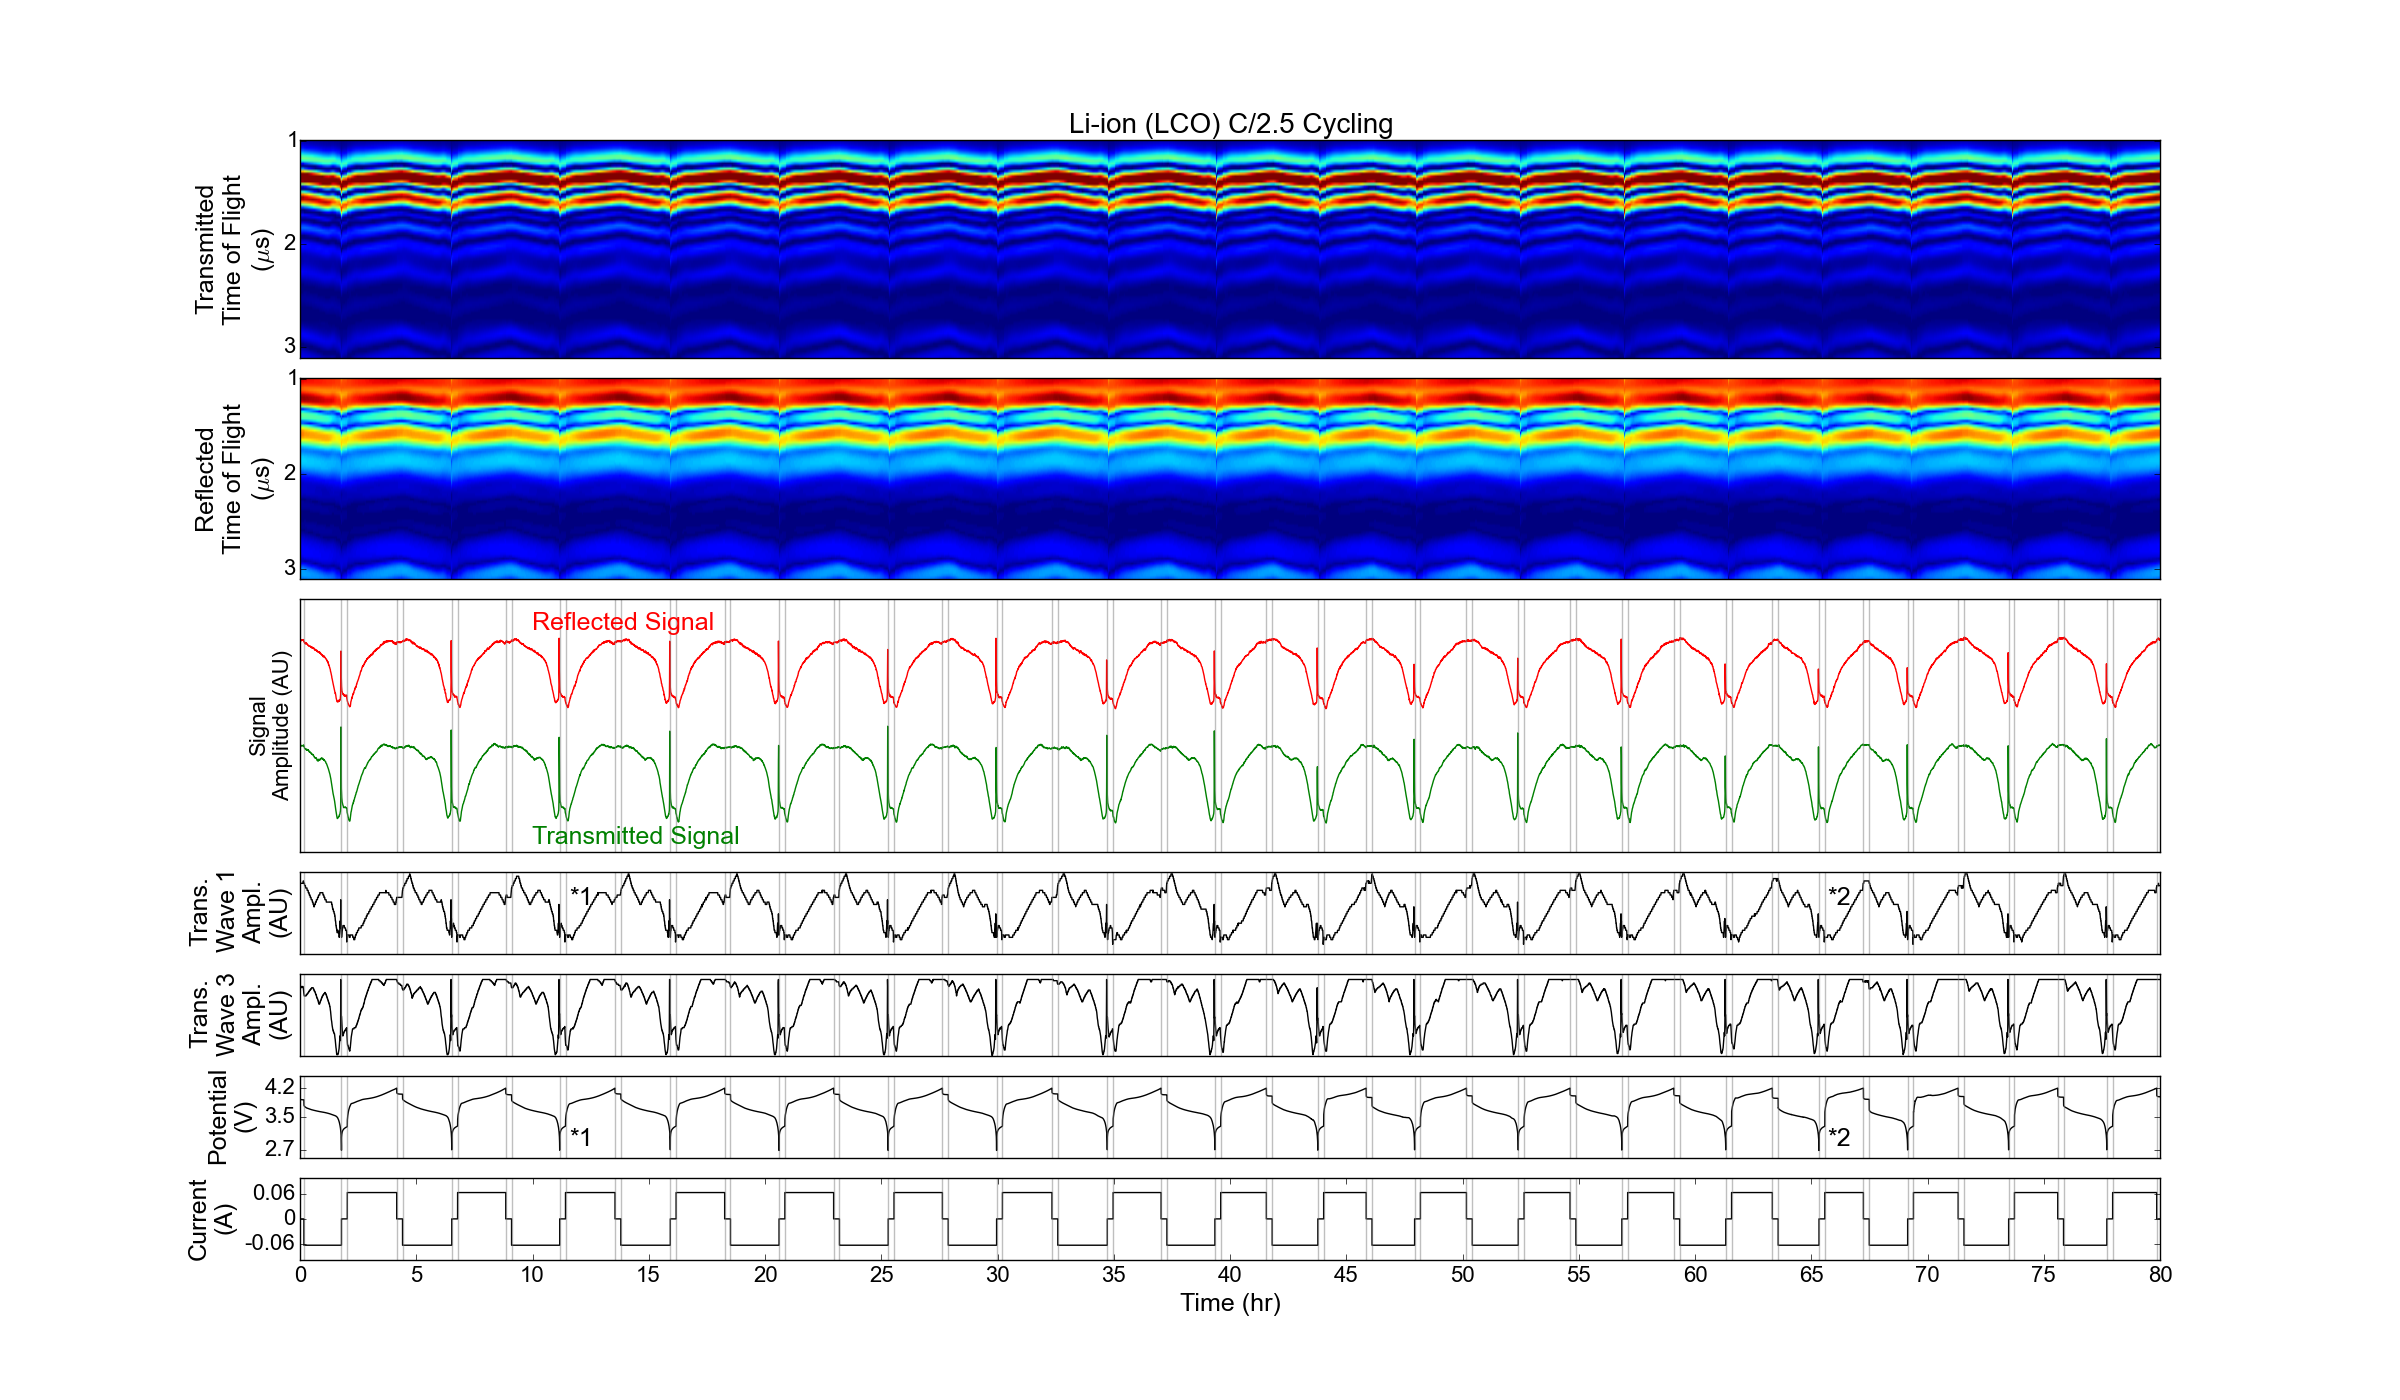
\includegraphics[width=\textwidth]{ch-appendices/images/lcofull.png}
    \caption[Full acoustic waveform of a \ce{LiCoO2}/graphite prismatic cell.]{Full acoustic waveform of a \ce{LiCoO2}/graphite prismatic cell. \textbf{(a,b)} ToF maps for transmission and reflection modes, respectively, \textbf{(c)} total reflected (red) and transmitted (green) signal amplitudes, \textbf{(d,e)} traces for the amplitudes of transmitted waves 1 and 3, respectively, \textbf{(f)} cell potential, and \textbf{(g)} applied current as a function of cycling time. The vertical gray lines in panels c-g represent transitions between charge, discharge, and rest steps; arrows 1, 3, and 10 as well as markings *1 and *2 are discussed in the text.}
    \label{fig:lcofull}
\end{figure} 

\section{NCA jelly roll cell}

\begin{figure}[htb]
  \centering
    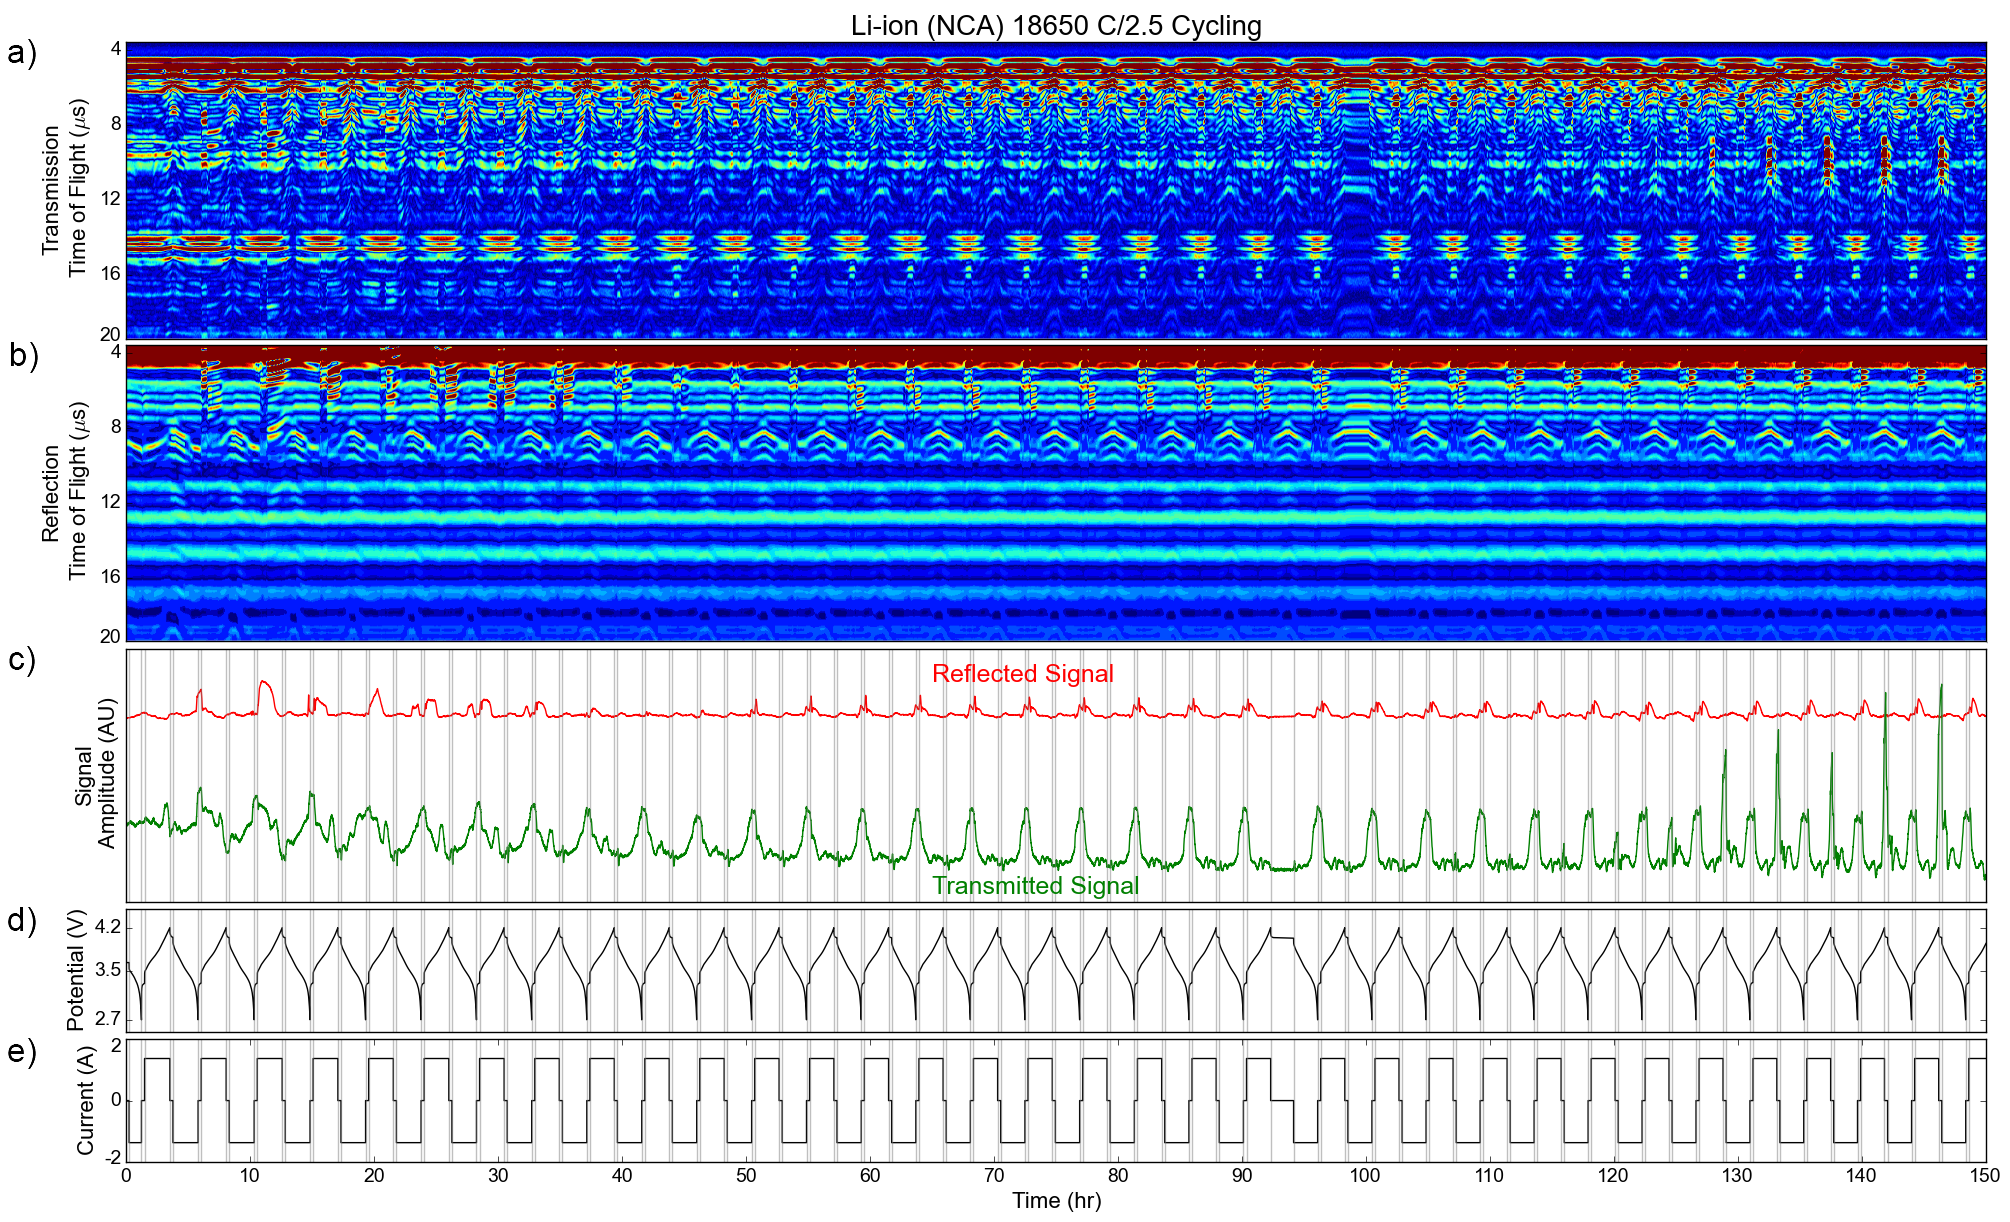
\includegraphics[width=\textwidth]{ch-appendices/images/ncafull.png}
    \caption[Full data set from Fig. 4: acoustic behavior of NCA/graphite 18650 cell.]{Full data set from Fig. 4: acoustic behavior of NCA/graphite 18650 cell. \textbf{(a,b)} ToF maps for transmission and reflection modes, respectively, \textbf{(c)} total reflected (red) and transmitted (green) signal amplitudes, \textbf{(d)} cell potential, and \textbf{(e)} applied current as a function of cycling time. An extra one hour rest step was added around hour 96 of testing. The vertical gray lines in panels c-e represent transitions between charge, discharge, and rest steps.}
    \label{fig:ncafull}
\end{figure}  